\documentclass[usenames,dvipsnames]{beamer}

\usepackage{tikz}
\usepackage{amsmath}
\usepackage{listings}
\usepackage{graphicx}
\usepackage{inconsolata}
\usetheme{LANL}
\usetikzlibrary{positioning}
\usetikzlibrary{shapes.misc}
\graphicspath{{./figs/}}
\usepackage{xcolor}

\lstset{
  basicstyle=\footnotesize\ttfamily,
  breaklines=true,
  moredelim=**[is][\color{BurntOrange}]{@}{@},
  moredelim=**[is][\color{RoyalBlue}]{&}{&},
}
\definecolor{myLightGray}{RGB}{192,192,192}
\setbeamercolor{fakegraphic}{bg=myLightGray,fg=black}

\title{In Situ Optimization and Late Lowering of Compute Kernels}

\date{March 2, 2022}
\author[shortname]{\textbf{George Stelle} \\ Pat McCormick, Daniel Shevitz,
Alexis Perry-Holby, Nirmal Prajapati \\ T.B. Schardl, Valentin Churavy}

\institute[shortinst]{Los Alamos National Laboratory}
          
\begin{document}

\begin{frame}
\maketitle
\end{frame}

\begin{frame}[fragile]
\frametitle{Compiler View}
\begin{columns}
\begin{column}{0.3\textwidth}
\begin{center}
COMPUTE KERNEL 
\end{center}
\end{column}
\begin{column}{0.3\textwidth}
\begin{center}
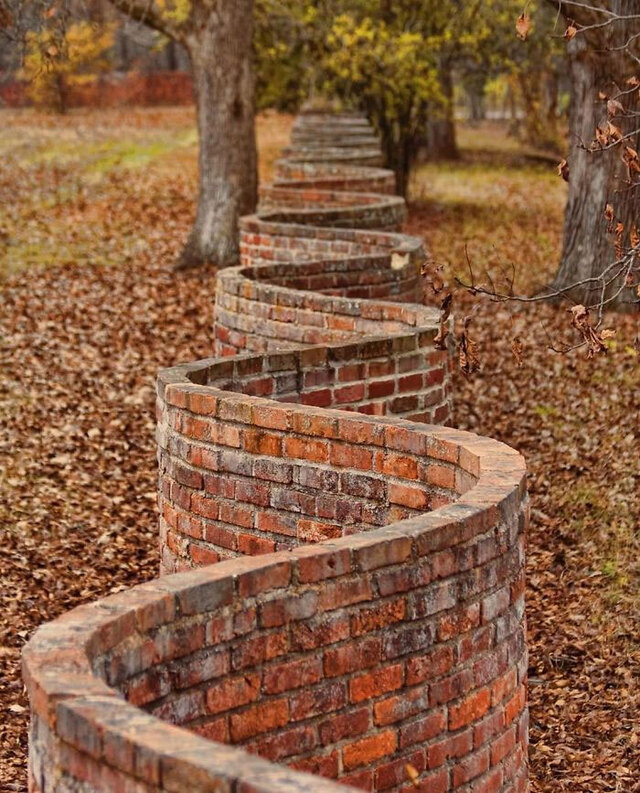
\includegraphics[width=\textwidth]{wall.jpg}
\end{center}
\end{column}
\begin{column}{0.3\textwidth}
\begin{center}
OTHER CODE
\end{center}
\end{column}
\end{columns}
\end{frame}

\begin{frame}[fragile]
\frametitle{Goal}
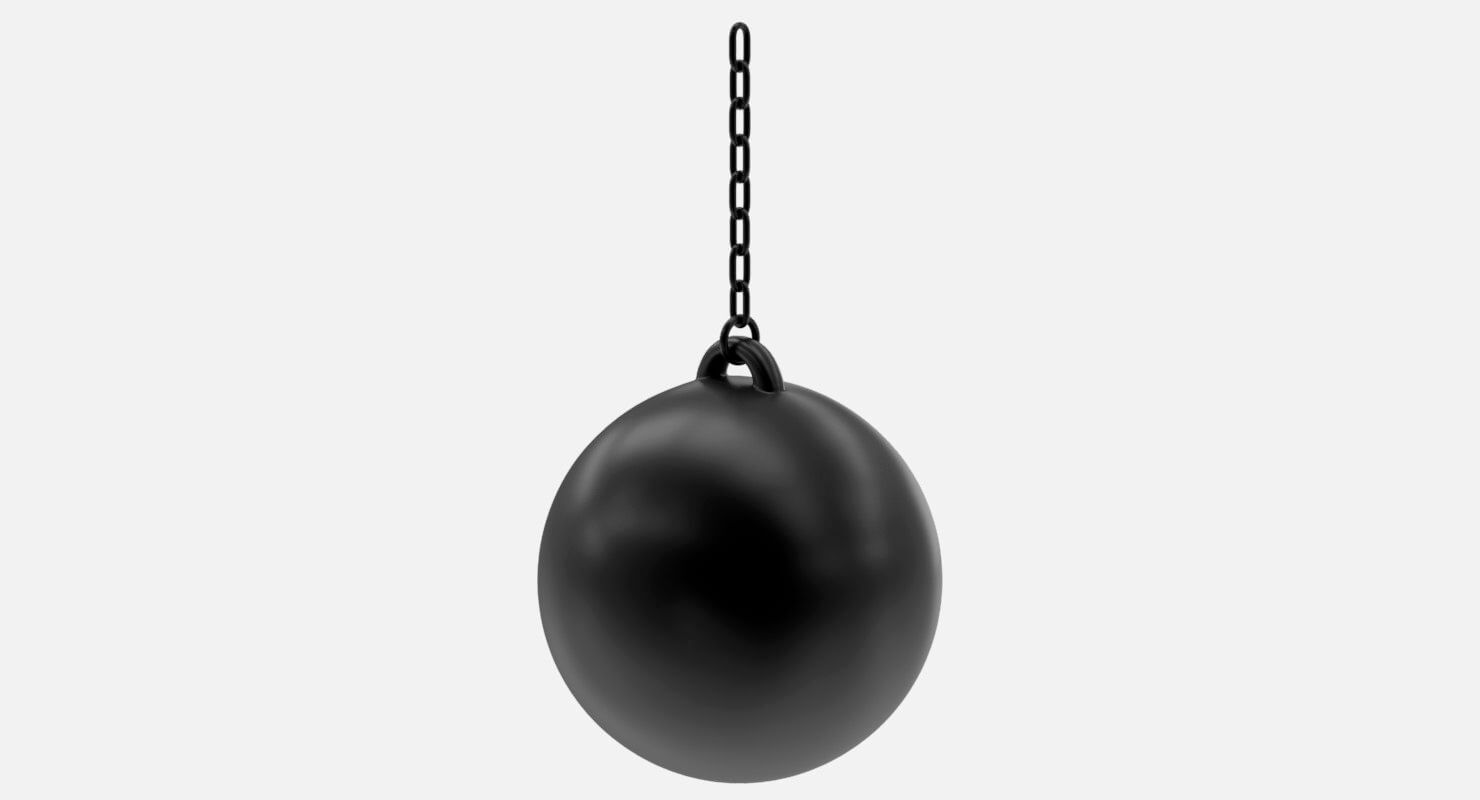
\includegraphics[width=\textwidth]{wreckingball.jpg}
\end{frame}


\begin{frame}[fragile]
\frametitle{LLVM}
\center
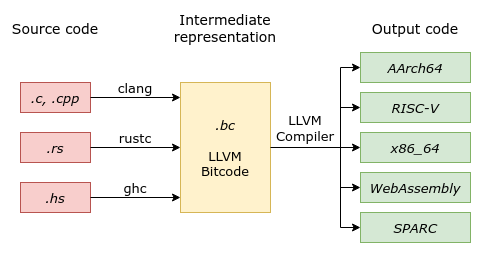
\includegraphics[width=\textwidth]{llvm.png}
\end{frame}

\begin{frame}[fragile]
\frametitle{Parallelism}
\center
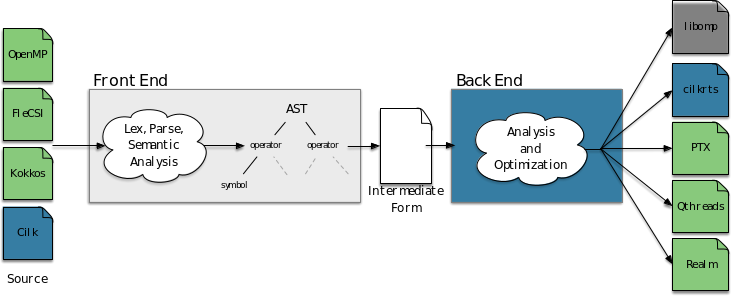
\includegraphics[width=\textwidth]{overview.png}
\end{frame}

\begin{frame}[fragile]
\frametitle{Accelerators}
\begin{columns}
\begin{column}{0.5\textwidth}
\center\textbf{Our Approach}

\begin{itemize}
\item Compile parallel loops into Tapir
\item Optimize!
\item Outline kernel, store as LLVM
\item Insert calls to libllvm-gpu
\item JIT compile kernel based on available devices
\end{itemize}
\end{column}
\begin{column}{0.5\textwidth}

\center
\textbf{Legacy Approach}
\vspace{1cm}
\begin{itemize}
\item Split compute kernel into separate compilation unit
\item Optimize independently
\item Lower to vendor ISA
\item Insert calls to vendor runtime 
\end{itemize}
\end{column}
\end{columns}
\end{frame}

\begin{frame}[fragile]
\frametitle{(Very) Preliminary Results}
\hspace{0.25\textwidth} 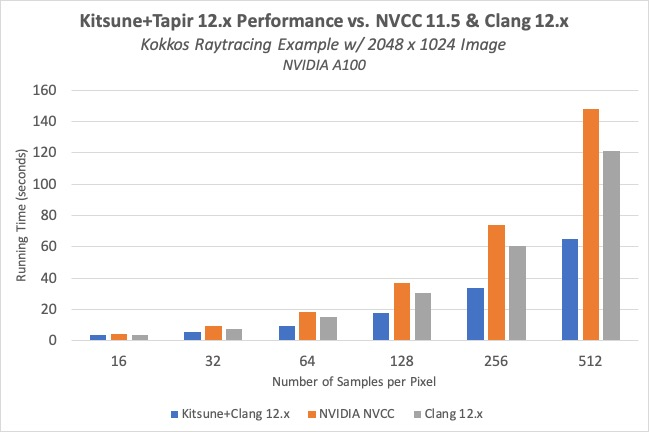
\includegraphics[width=0.5\textwidth]{results.jpg}
\end{frame}

\begin{frame}[fragile]
\frametitle{In Progress}
\begin{itemize}
\item Reductions
\item SSA Theory Extensions
\item Better JIT Utilization
\item Explicit Memory Movement
\item Precompilation
\end{itemize}
\end{frame}

\begin{frame}
\center
\huge{Questions?}\\
\vspace{2cm}
\small
\texttt{https://github.com/lanl/kitsune}\\
\texttt{stelleg@lanl.gov} 
\end{frame}

\end{document}

